\documentclass{article}

\usepackage{graphicx}
\usepackage{bbm}
\usepackage{amsmath}
\usepackage{amssymb}
\usepackage{filecontents}
\usepackage{amsthm}
\usepackage{mathrsfs}
\usepackage{amssymb}
\usepackage{amsfonts}
\usepackage{authblk}
\usepackage{hyperref}
\hypersetup{
    colorlinks=true,
    linkcolor=blue,
    filecolor=magenta,      
    urlcolor=cyan,
}
\def\<#1>{\left\langle #1 \right\rangle}
%
\newcommand{\N}{\ensuremath{\mathbbm{N}}}
\newcommand{\Z}{\ensuremath{\mathbbm{Z}}}
\newcommand{\Q}{\ensuremath{\mathbbm{Q}}}
\newcommand{\R}{\ensuremath{\mathbbm{R}}}
\newcommand{\C}{\ensuremath{\mathbbm{C}}}
\newcommand{\CP}{\ensuremath{\mathbbm{CP}}}
\renewcommand{\H}{\ensuremath{\mathbbm{H}}}
\newcommand{\F}{\ensuremath{\mathcal{F}}}

\newcommand{\ci}{\ensuremath{\mathrm{i}}}
\newcommand{\qi}{\ensuremath{\mathbbm{i}}}
\newcommand{\qj}{\ensuremath{\mathbbm{j}}}
\newcommand{\qk}{\ensuremath{\mathbbm{k}}}

\DeclareMathOperator*{\argmin}{arg\,min}

\newcommand{\J}{\mathbf{J}}
\newcommand{\K}{\mathbf{K}}
\newcommand{\x}{\mathbf{x}}
\newcommand{\D}{\mathscr{D}}
\newcommand{\M}{\mathbf{M}}
%\newcommand{\u}{\mathscr{u}}
%\newcommand{\v}{\mathscr{v}}
\newcommand{\TD}{\ensuremath{T_{V(t)}\D}}
\newcommand{\ND}{\ensuremath{N_{V(t)}\D}}

\newtheorem{theorem}{Theorem}[section]
\newtheorem{corollary}{Corollary}[theorem]
\newtheorem{lemma}[theorem]{Lemma}
\theoremstyle{definition}
\newtheorem{definition}{Definition}[section]
%

\title{Curved Folded Wallpapers}
\author[1]{Michael Rabinovich}
\begin{document}

\maketitle

\section{Curved folded DOGs}

This document discuss various ideas on optimizing for and simulating curved folding on DOGs, though the techniques might be relevant for developable surfaces in general.

\section{Smooth curved folds}
Given a curve $\gamma$ in $\mathbb{R}^3$ and a non straight flattening of the curve $\gamma_{2d}$, there are exactly 2 different developable surfaces going through that curve with the same flattening of that curve,. A choice of 2 different ones, denoted as $S_1,S_2$ from each side is said to be a fold along that curve.

\begin{figure} [h]
	\centering
	\includegraphics[width=0.7\linewidth]{curved_fold_through_curve.pdf}
	\caption{Left: A flattened curve in 2D. Right: A small neighbourhood around an embedding of the curve in $\mathbb{R}^3$, and 2 different developable surfaces passing through the curve, such that the tangent plane on the curve is different from each side.}
	\label{fig:curved_fold_through_curve}
\end{figure}

\subsection{Local frame around a curve on a developable}
Through this note we will use the local Frenet frame around a curve $\gamma$ on a developable (or DOG), denoting it as $F = \{t,n,b\}$ for the tangent, principal normal and the binormal.
	
\subsection{Characterization 1: Reflection of tangent planes}
Along a curved fold the curves osculating plane bisects the tangent planes of the 2 developables passing through the curve. The dihedral fold angles between the developables is dependant on the bending of the surface along the curve. The more the surface is bend along that curve, the bigger the fold is. Precisely, if at a given point the curvature of the embedding in $3d$ is $k(t)$, its original flattened curvature (or geodesic curvature) is $k_g(t) = cos(\alpha)k(t)$ and the its normal curvature (measuring the bending of that curve) is $k_n(t) = sin(\alpha)k(t)$, then the dihedral folding angle between along the fold is $2\alpha$. The fact that the curve's osculating plane bisects the tangent planes means that along a curved fold, the tangent plane is reflected through the osculating plane, as opposed to being equal when there is no fold and the curve lies on a smooth developable surfaces.

\subsection{Characterization 2: Rotations of tangents around the curve}
One can also look at the previous characterization of a fold as a rotation of tangent vectors from one side of the developable surface by an angle of $2\alpha$ around the curve's tangent. This creates discontinuity between tangents of the surface from each side. The angle of the rotated tangents depends on the initial angle between the flattenend tangent and the curve's tangent. For instance if they are orthogonal, the angle between the rotated tangent is the same as the angle between the normals of both surfaces. If they are parallel to the curve, than its 0.

\subsection{Characterization 3: Side of osculating plane}
The previous characterizations implies that if $t_1$ is a vector of the tangent space of $S_1$ along a point on $\gamma$ than the "continuation" of that tangent from the other side of the surface at $S_2$ satisfies $\langle <t_1,b> \rangle = -\langle <t_2,b> \rangle$ if $b$ is the binormal of the curve at that point. This is opposed to the equality $\langle <t_1,b> \rangle = \langle <t_2,b> \rangle$ when there is no fold. This gives us a more "binary" charecterization of folded vs. non folded configuration along a curve. A developable surface is curved folded along a curve if it lies on the same side of the osculating plane of the curve. Otherwise, each $S_1,S_2$ lie on a different side. TODO: add drawing.
This might be important for optimization, as we can't probably expect to have the previous conditions satisfied exactly on a discrete DOG along an entire curve, but we can expect the sign/side of plane to be correct.

\begin{figure} [h]
	\centering
	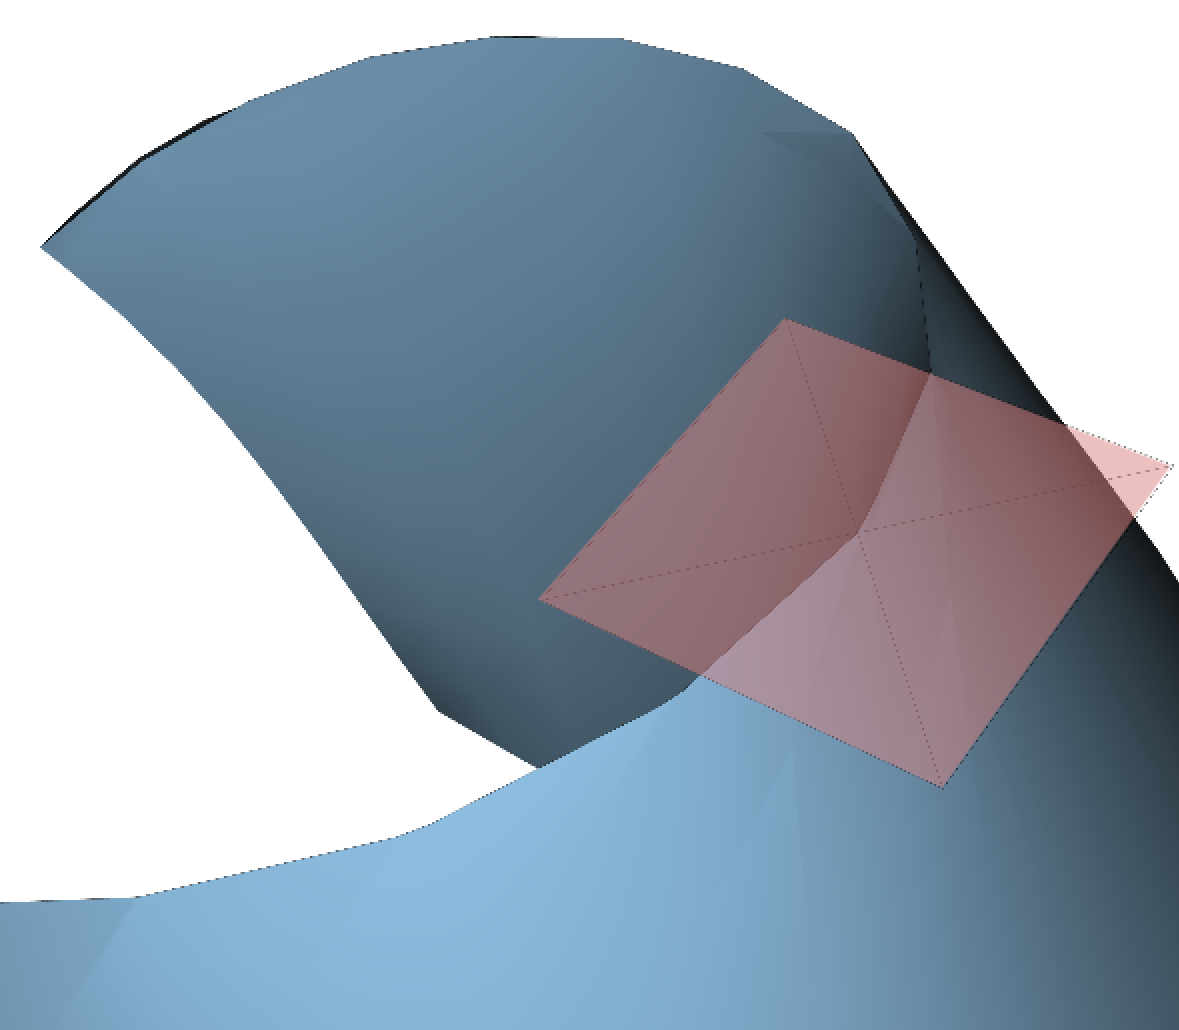
\includegraphics[width=0.5\linewidth]{plane_side}
	\caption{Both surfaces are at the same side of the osculating plane in a curved fold. If the surface was not curved folded, the osculating plane would have intersect the surface.}
	\label{fig:curved_fold_through_curve}
\end{figure}

\subsection{Mountain and Valley folds}
A fold is said to be a mountain fold according to the angles between $t_1,b$ or equivalently by the angle between $t_2,b$.

\subsection{Multiple curved folds}
Deforming the curve fold locally deform the entire surface. This (generally) further cause deformation of other curved folds if they exist. For instance for multiple patterns one can choose whether to fold valley/mountain only on 1 fold, and the rest is determined automatically. Similarly if we assign dihedral angles along one fold, this might constrain the dihedral angles around another fold. Thus we should be careful when assigning folding constraint as there is a dependency between different folds.

\begin{figure} [h]
	\centering
	\includegraphics[width=\linewidth]{multiple_curve_pattern}
	\caption{A curved folded pattern with multiple creases. Changing the curve between A to B affects the shape of C. All the parameters, folding angles, curvatures/torsions, are linked constrained together.}
	\label{fig:folding_an_edge.pdf}
\end{figure}
	
\section{Optimizing for curved folds on DOGs}
\subsection{Discrete fold}

\begin{figure} [h]
	\centering
	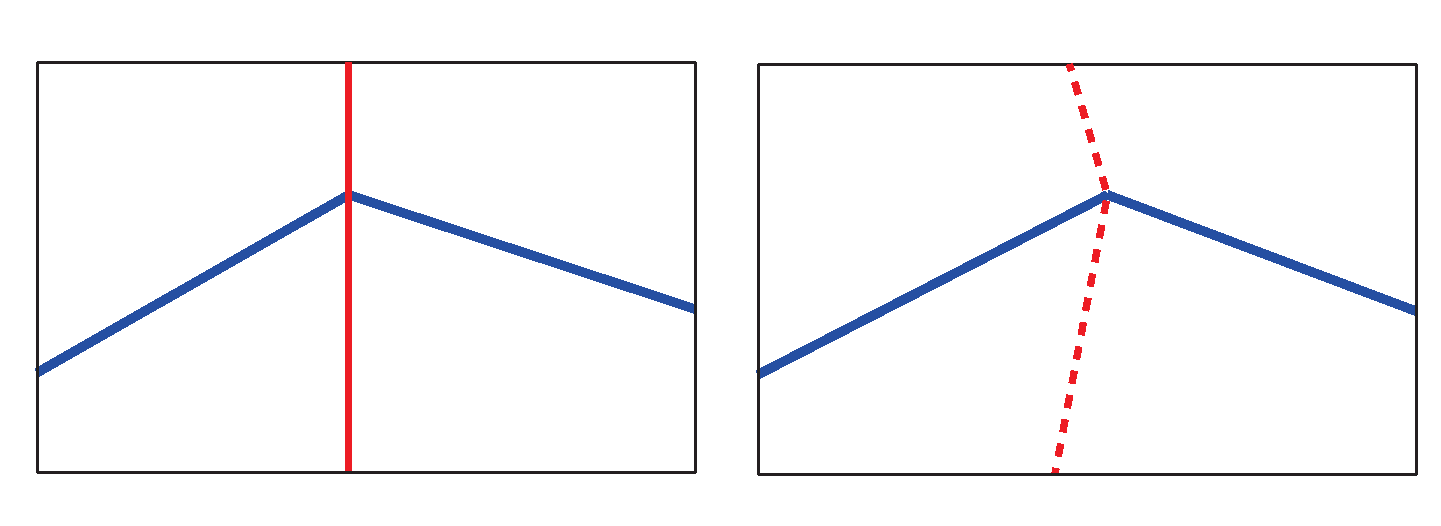
\includegraphics[width=0.5\linewidth]{folding_an_edge.pdf}
	\caption{We represent curved folds on DOGs by using different connected component around a curve (here in blue), essentially duplicating shared quads. The red edge is a tangent. On a flat configuration it is continues, or straight from both sides, while a fold is a discontinuity of the tangent created by rotating the tangents along the tangent of the blue curve as explained above, or equivalently in the smooth case by reflecting one tangent along the osculating plane of the blue curve.}
	\label{fig:folding_an_edge.pdf}
\end{figure}
The red curve can be seen as a tangent from each surface. On a curved conifguration its not colinear, and any discretization for the Frenet frame on the blue curve can be used.

\subsection{One fold using positional constraints}
The easiest way to fold a single curve, is by prescribing positional constraints along one point  of the curved fold, and then minimize bending + isometry objective on a DOG. We can derive positional constraints by simply fixing that point, and rotating the tangent of both surfaces around the tangent of the curve by an angle. Then slowly increasing this angle creates a fold. The ratio between the tangents angle and the dihedral folding angle is dependant of the angle of the flattened tangent with the curve's tangent (and is something I've written on the board), in case we want to prescribe a dihedral angle.

\subsubsection{Positional constraints - Difficulties in extending for multiple folds}
The problem in extending this fold to multiple one is compatability of different folds. One cannot fix two points along to different folds and still fold it for instance. If we don't fix the second point, it's also not very clear how to derive the positional constraints along a second curve.

\subsection{Folding movement and folding bias}
At best, instead of a folding movement we could get a folding bias. So not only some way to fold a paper, but have an objective with a possible set of constraints that can be added to some deformation guaranteeing or pushing towards folded configuration. This will allow us for instance to deform a curve while folding the entire surface simultaneously.

\subsection{Knowing M/V assignemnt}
Some discretization that will be shown below can be made easier if we know upfront the M/V assignment of the folds. This is in general not known for arbitrary folds but can be easily tested for known crease patterns. Furthermore, if such a discretization will work well we could consider a precomputation of finding a valid/good M/V assignment.

\subsection{Equalities and inequalities}
Characterization 1/2 can be discretized using equality constraints by requiring around a fold that  $\langle t_1,b \rangle = -\langle t_2,b \rangle$ for some discretization of $b$, and using $t_!,t_2$ as the two sides of the red edge in the figure. This is an equality constraint. Alternatively, charecterization 3 can be discretized by merely asking for $\langle t_1,b \rangle \langle t_2,b \rangle < 0$. If we know the mountain/valley assignment this constraint becomes easier, in the form of $\langle t_1,b \rangle < 0$ or $\langle t_1,b \rangle > 0$ from both sides (depending on the sign of $t_1$ and on the M/V assignment).

\subsection{Equality folding constraints}
The first problem with the above mentioned equality constraints is that they are not 'exact'. We can't hope to satisfy all of them exactly (or numerically). Thought we can expect a low deviation. Practically this means that the Jacobian of the constraints, if we'll use it, will probably be rank deficient. We could then perform a QR on the constraints to remove linear dependant constraints, but this also means that we need to remove the appropriate rhs constraint values, and in general we cannot hope to achieve that or have a well defined optimization problem. Putting these constraints at the objective brings as to the problem of choosing the appropriate weight for the constraints, which will compete the bending and isometry objective, or the other positional constraints of the curve.

\subsection{Inequality folding constraints}
The inequality point of view is useful, as folding/not folding is in fact a binary choice in the smooth case which is done exactly at the beginning of the deformation. After a finite timestep, we cannot undone a folding unless we flattened that part. Optimizing with inequalities is typically done either using barrier methods or active-set methods. 
\subsubsection{Active set methods}
In terms of active-set terminology, our optimization is quite unique. All the inequalities start active, and we actually know that we want the active set to be empty. The first problem is that the constraints are almost likely linearly dependent and the first steps means we should include them as equalities. The second and bigger problem is that on the one hand we know that the active set is zero, but minimizing bending energy will probably incur no folds. We are most likely not looking for a KKT point with just the bending energy, at least before the paper was folded "enough", at that point the folds or continuity along them stay the same anyhow. The problem is in fact not well defined by just using bending energy, which unfortunately probably means the minimum is not bounded (might be that at first steps the KKT point actually has equalities...).

\subsubsection{Barrier methods}
The KKT argument issue as written in "Active set methods" is probably the same there. I've implemented some barrier method and it didn't work. Also, the first step also doesn't lead to feasibility in the constraints. Another problem here is that as opposed to the equality constraint problem, we don't start from a minimum of the energy. We start with infinite energy as all the constraints are active.

\section{Things to try}
1) Equality constraints for 1 point in each curve.\\
2) Equality constraints penalty for each point on a curve. Make it strong enough such that we always stay feasible (by changing the weight). Not clear what's the optimization problem we solve here. \\
3) Combine 1 with 2. \\
4) Equality constraints on all points in every curve, and then use QR. \\
5) Smarter positional constraints. Then the problem should be well defined? We can use local Frenet frames. The tangent angle can be defined based on the curve's curvature, torsion, and initial geoedesic curvature. Under isometry assumption the tangent and principal normal should be linear. This requires M/V assignment.

%\section{Appendix}

%\clearpage%ss
%\bibliographystyle{plain}
%\bibliography{97-bib-opt}
\end{document}
